\documentclass[aspectratio=169]{beamer}

% Suppress the navigation bar
\beamertemplatenavigationsymbolsempty

% Change the font
\usepackage{fontspec}
\setmainfont{DejaVu Serif}
\setsansfont{DejaVu Sans}
\setmonofont{DejaVu Sans Mono}
\setbeamerfont{title}{series=\bfseries}
\setbeamerfont{frametitle}{series=\bfseries}

% Change the themes
\usecolortheme[accent=blue, dark]{solarized}
\useinnertheme{circles}
\setbeamercolor{item projected}{bg=solarizedRebase0, fg=solarizedRebase03}
\setbeamercolor{solarizedcolorbox}{bg=solarizedRebase02, fg=solarizedRebase0}

% Custom packages
\usepackage{listings}
\usepackage{tikz}
\usetikzlibrary{arrows,automata,positioning}
\newenvironment{fsa}{\begin{center}
\begin{tikzpicture}[shorten >=1pt, initial text=]
  \tikzstyle{every state}=[draw=solarizedAccent, node distance=2cm,
                           minimum size=1cm]
  \tikzstyle{accepting}=[double=solarizedRebase03]}{\end{tikzpicture}
\end{center}}

% Custom title page
\defbeamertemplate*{title page}{customized}[1][]
{ 
  \begin{flushright}
    {\usebeamerfont{institute}\insertinstitute}
  \end{flushright}
  \begin{beamercolorbox}[wd=\paperwidth, sep=2em]{solarizedcolorbox}
    {\usebeamerfont{title}\usebeamercolor[fg]{title}\inserttitle}
  \end{beamercolorbox}
  \begin{flushright}
    {\usebeamerfont{author}\insertauthor}

    {\usebeamerfont{institute}\insertdate}
  \end{flushright}
}

\title{Lexing and Parsing}
\author{Jon Eyolfson}
\date{May 31, 2013}
\institute{University of Waterloo}

\begin{document}
%%%%%%%%%%%%%%%%%%%%%%%%%%%%%%%%%%%%%%%%%%%%%%%%%%%%%%%%%%%%%%%%%%%%%%%%%%%%%%%%
\begin{frame}[plain, noframenumbering]
  \titlepage
\end{frame}
%%%%%%%%%%%%%%%%%%%%%%%%%%%%%%%%%%%%%%%%%%%%%%%%%%%%%%%%%%%%%%%%%%%%%%%%%%%%%%%%

%%%%%%%%%%%%%%%%%%%%%%%%%%%%%%%%%%%%%%%%%%%%%%%%%%%%%%%%%%%%%%%%%%%%%%%%%%%%%%%%
\begin{frame}
\frametitle{Goal}

Formulate a grammar for integer arithmetic
\end{frame}
%%%%%%%%%%%%%%%%%%%%%%%%%%%%%%%%%%%%%%%%%%%%%%%%%%%%%%%%%%%%%%%%%%%%%%%%%%%%%%%%

%%%%%%%%%%%%%%%%%%%%%%%%%%%%%%%%%%%%%%%%%%%%%%%%%%%%%%%%%%%%%%%%%%%%%%%%%%%%%%%%
\begin{frame}
\frametitle{Backus-Naur Form}

BNF is a common way we formulate grammars\\~\\

Given as $G = (T, N, S, P)$, where:

\begin{description}
  \item[$G$] is the grammar
  \item[$T$] is a set of terminals
  \item[$N$] is a set of non-terminals
  \item[$S$] is the starting non-terminal
  \item[$P$] is a set of productions
\end{description}
\end{frame}
%%%%%%%%%%%%%%%%%%%%%%%%%%%%%%%%%%%%%%%%%%%%%%%%%%%%%%%%%%%%%%%%%%%%%%%%%%%%%%%%

%%%%%%%%%%%%%%%%%%%%%%%%%%%%%%%%%%%%%%%%%%%%%%%%%%%%%%%%%%%%%%%%%%%%%%%%%%%%%%%%
\begin{frame}
\frametitle{Terminals}

A \alert{terminal} is usually a \alert{token} from the \alert{lexer}\\~\\

A \alert{token} is a group of characters with a single meaning\\~\\

\begin{beamercolorbox}[sep=1em]{solarizedcolorbox}
  The \alert{lexer} is responsible for enforcing these groupings and stripping
  out white space
\end{beamercolorbox}

\end{frame}
%%%%%%%%%%%%%%%%%%%%%%%%%%%%%%%%%%%%%%%%%%%%%%%%%%%%%%%%%%%%%%%%%%%%%%%%%%%%%%%%

%%%%%%%%%%%%%%%%%%%%%%%%%%%%%%%%%%%%%%%%%%%%%%%%%%%%%%%%%%%%%%%%%%%%%%%%%%%%%%%%
\begin{frame}
\frametitle{Tokens}

There are two types of tokens: simple and compound\\~\\

A \alert{simple token} is usually a single character\\~\\

A \alert{compound token} is defined by a \alert{regular expression}\\~\\

Note that we can query the string which matched a token
\end{frame}
%%%%%%%%%%%%%%%%%%%%%%%%%%%%%%%%%%%%%%%%%%%%%%%%%%%%%%%%%%%%%%%%%%%%%%%%%%%%%%%%

%%%%%%%%%%%%%%%%%%%%%%%%%%%%%%%%%%%%%%%%%%%%%%%%%%%%%%%%%%%%%%%%%%%%%%%%%%%%%%%%
\begin{frame}
\frametitle{Our Tokens}

Simple: $+, -, *, /$\\~\\

Compound: \lstinline{INT}\\~\\~\\

Therefore, $T = \{ +, -, *, /,$\lstinline{INT}$\}$
\end{frame}
%%%%%%%%%%%%%%%%%%%%%%%%%%%%%%%%%%%%%%%%%%%%%%%%%%%%%%%%%%%%%%%%%%%%%%%%%%%%%%%%

%%%%%%%%%%%%%%%%%%%%%%%%%%%%%%%%%%%%%%%%%%%%%%%%%%%%%%%%%%%%%%%%%%%%%%%%%%%%%%%%
\begin{frame}[plain, noframenumbering]
  \begin{beamercolorbox}[wd=\paperwidth, sep=2em]{solarizedcolorbox}
    {\usebeamerfont{title}\usebeamercolor[fg]{title} \hfill Start Lexing}
  \end{beamercolorbox}
\end{frame}
%%%%%%%%%%%%%%%%%%%%%%%%%%%%%%%%%%%%%%%%%%%%%%%%%%%%%%%%%%%%%%%%%%%%%%%%%%%%%%%%

%%%%%%%%%%%%%%%%%%%%%%%%%%%%%%%%%%%%%%%%%%%%%%%%%%%%%%%%%%%%%%%%%%%%%%%%%%%%%%%%
\begin{frame}
\frametitle{Regular Expression Operations}

Recall a \alert{regular expression} is made up of characters and the following
operators:

\begin{center}
\begin{tabular}{cl}
$\cdot$        & sequence (implied)\\
\lstinline{[]} & character sets\\
\lstinline{|}  & alternation (left or right)\\
\lstinline{()} & grouping\\
\lstinline{*}  & repetition (zero or more)\\
\lstinline{+}  & repetition (one or more)\\
\lstinline{?}  & repetition (zero or one)\\
\end{tabular}
\end{center}

The repetition operators apply to the preceding element
\end{frame}
%%%%%%%%%%%%%%%%%%%%%%%%%%%%%%%%%%%%%%%%%%%%%%%%%%%%%%%%%%%%%%%%%%%%%%%%%%%%%%%%

%%%%%%%%%%%%%%%%%%%%%%%%%%%%%%%%%%%%%%%%%%%%%%%%%%%%%%%%%%%%%%%%%%%%%%%%%%%%%%%%
\begin{frame}
\frametitle{Regular Expression Output}

When we apply a \alert{regular expression} to a string and it will match or
not\\~\\

\begin{center}
\begin{tabular}{lll}
\bfseries Regular Expression & \bfseries String &  \bfseries Match\\
\lstinline{aa*}    &                & No\\
\lstinline{a+}     & \lstinline{a}  & Yes\\
\lstinline{a+}     & \lstinline{aa} & Yes\\
\lstinline{(ab)|b} & \lstinline{a}  & No\\
\lstinline{a?b}    & \lstinline{b}  & Yes\\
\lstinline{a?b}    & \lstinline{ab} & Yes\\
\end{tabular}
\end{center}
\end{frame}
%%%%%%%%%%%%%%%%%%%%%%%%%%%%%%%%%%%%%%%%%%%%%%%%%%%%%%%%%%%%%%%%%%%%%%%%%%%%%%%%

%%%%%%%%%%%%%%%%%%%%%%%%%%%%%%%%%%%%%%%%%%%%%%%%%%%%%%%%%%%%%%%%%%%%%%%%%%%%%%%%
\begin{frame}
\frametitle{Formulating an Integer}

Recall, we need to define the \lstinline{INT} \alert{token} (or
\alert{terminal}) for our grammar\\~\\

We would verbally describe it as one or more digits
\end{frame}
%%%%%%%%%%%%%%%%%%%%%%%%%%%%%%%%%%%%%%%%%%%%%%%%%%%%%%%%%%%%%%%%%%%%%%%%%%%%%%%%

%%%%%%%%%%%%%%%%%%%%%%%%%%%%%%%%%%%%%%%%%%%%%%%%%%%%%%%%%%%%%%%%%%%%%%%%%%%%%%%%
\begin{frame}
\frametitle{Regular Expression for Integers}

We would use the character set \lstinline{[0-9]} to match a single digit\\~\\

Since we want one or more digits, we can apply \lstinline{+} to a digit\\~\\

Giving us the regular expression \lstinline{[0-9]+}
\end{frame}
%%%%%%%%%%%%%%%%%%%%%%%%%%%%%%%%%%%%%%%%%%%%%%%%%%%%%%%%%%%%%%%%%%%%%%%%%%%%%%%%

%%%%%%%%%%%%%%%%%%%%%%%%%%%%%%%%%%%%%%%%%%%%%%%%%%%%%%%%%%%%%%%%%%%%%%%%%%%%%%%%
\begin{frame}
\frametitle{Regular Expression Application}

How do regular expression implementations actually work?\\~\\

One way is to convert the regular expression to a \alert{finite state automaton}
(FSA) and apply the input character by character
\end{frame}
%%%%%%%%%%%%%%%%%%%%%%%%%%%%%%%%%%%%%%%%%%%%%%%%%%%%%%%%%%%%%%%%%%%%%%%%%%%%%%%%

%%%%%%%%%%%%%%%%%%%%%%%%%%%%%%%%%%%%%%%%%%%%%%%%%%%%%%%%%%%%%%%%%%%%%%%%%%%%%%%%
\begin{frame}
\frametitle{Finite State Automaton}

A FSA contains the following:
\begin{itemize}
  \item A set of \alert{states} and \alert{state transitions}
  \item A \alert{initial state} and one or more \alert{accepting states}\\~\\
\end{itemize}

\alert{States} are arbitrarily numbered and \alert{state transitions} are for
individual characters
\end{frame}
%%%%%%%%%%%%%%%%%%%%%%%%%%%%%%%%%%%%%%%%%%%%%%%%%%%%%%%%%%%%%%%%%%%%%%%%%%%%%%%%

%%%%%%%%%%%%%%%%%%%%%%%%%%%%%%%%%%%%%%%%%%%%%%%%%%%%%%%%%%%%%%%%%%%%%%%%%%%%%%%%
\begin{frame}
\frametitle{FSA Notation}

\begin{fsa}
  \node[state]                                 (sn)               {$s_n$};
  \node[state, initial]                        (s0) [right=of sn] {$s_0$};
  \node[state, accepting, node distance=2.5cm] (s1) [right=of s0] {$s_1$};
  \node[below of=sn] {State $n$};
  \node[below of=s0] {Initial state};
  \node[below of=s1] {Accepting state}; 
\end{fsa}

\alert{State transitions} are represented by labelled arrows
\end{frame}
%%%%%%%%%%%%%%%%%%%%%%%%%%%%%%%%%%%%%%%%%%%%%%%%%%%%%%%%%%%%%%%%%%%%%%%%%%%%%%%%

%%%%%%%%%%%%%%%%%%%%%%%%%%%%%%%%%%%%%%%%%%%%%%%%%%%%%%%%%%%%%%%%%%%%%%%%%%%%%%%%
\begin{frame}
\frametitle{FSA Usage}

To match a string with our \alert{regular expression}, do the following:\\~\\

\begin{enumerate}
  \item Begin at the initial state\\~\\
  \item Take the \alert{state transition} matching the current character
    \begin{itemize}
      \item If no transition, string does not match\\~\\
    \end{itemize}
  \item Repeat step 2 for the next character until there are no more\\~\\
  \item Check if we're in an accepting state

    \begin{itemize}
      \item If so, the string does match
      \item Otherwise, string does not match
    \end{itemize}
\end{enumerate}
\end{frame}
%%%%%%%%%%%%%%%%%%%%%%%%%%%%%%%%%%%%%%%%%%%%%%%%%%%%%%%%%%%%%%%%%%%%%%%%%%%%%%%%

\newcommand{\fsausage}{\begin{fsa}
  \node[state,initial]   (s0)               {$s_0$};
  \node[state,accepting] (s1) [right=of s0] {$s_1$};
  \path[->] (s0) edge node[above] {\lstinline{\a}} (s1);
  
\end{fsa}}

%%%%%%%%%%%%%%%%%%%%%%%%%%%%%%%%%%%%%%%%%%%%%%%%%%%%%%%%%%%%%%%%%%%%%%%%%%%%%%%%
\begin{frame}
\frametitle{FSA Usage Question}

Consider the \alert{regular expression} \lstinline{a}\\~\\

This corresponds to the following FSA: 

\fsausage{}

Apply it to the following strings:

\begin{enumerate}
  \item \lstinline{a}
  \item $\varepsilon$ (fancy way of saying an empty string)
  \item \lstinline{bob}
\end{enumerate}

Which strings match, and which do not?
\end{frame}
%%%%%%%%%%%%%%%%%%%%%%%%%%%%%%%%%%%%%%%%%%%%%%%%%%%%%%%%%%%%%%%%%%%%%%%%%%%%%%%%

%%%%%%%%%%%%%%%%%%%%%%%%%%%%%%%%%%%%%%%%%%%%%%%%%%%%%%%%%%%%%%%%%%%%%%%%%%%%%%%%
\begin{frame}
\frametitle{FSA Usage Answer}

\fsausage{}

\begin{enumerate}
  \item \lstinline{a}
    \begin{itemize}
      \item Begin at state $s_0$
      \item Transition to $s_1$ with character \lstinline{a}
      \item No more characters, and in an accepting state
      \item \textbf{Match}
    \end{itemize} 
  \item $\varepsilon$
    \begin{itemize}
      \item Begin at state $s_0$
      \item No more characters, and not in an accepting state
      \item \textbf{No match}
    \end{itemize}
  \item \lstinline{bob}
    \begin{itemize}
      \item Begin at state $s_0$
      \item No transition with character \lstinline{b}
      \item \textbf{No match}
    \end{itemize}
\end{enumerate}
\end{frame}
%%%%%%%%%%%%%%%%%%%%%%%%%%%%%%%%%%%%%%%%%%%%%%%%%%%%%%%%%%%%%%%%%%%%%%%%%%%%%%%%

%%%%%%%%%%%%%%%%%%%%%%%%%%%%%%%%%%%%%%%%%%%%%%%%%%%%%%%%%%%%%%%%%%%%%%%%%%%%%%%%
\begin{frame}
\frametitle{FSA Conversions (1)}

\textbf{Regular Expression:} \lstinline{ab}

\begin{fsa}
  \node[state,initial] (s0)               {$s_0$};
  \node[state]         (s1) [right=of s0] {$s_1$};
  \node[state]         (s2) [right=of s1] {$s_2$};
  \path[->]
    (s0) edge node[above] {{\tt a}} (s1)
    (s1) edge node[above] {{\tt b}} (s2);
\end{fsa}
\end{frame}
%%%%%%%%%%%%%%%%%%%%%%%%%%%%%%%%%%%%%%%%%%%%%%%%%%%%%%%%%%%%%%%%%%%%%%%%%%%%%%%%

%%%%%%%%%%%%%%%%%%%%%%%%%%%%%%%%%%%%%%%%%%%%%%%%%%%%%%%%%%%%%%%%%%%%%%%%%%%%%%%%
\begin{frame}
\frametitle{FSA Conversions (2)}

\textbf{Regular Expression:} \lstinline{a|b}

\begin{fsa}
  \node[state,initial] (s0)               {$s_0$};
  \node[state]         (s1) [right=of s0] {$s_1$};
  \path[->]
    (s0) edge [bend left] node[above] {{\tt a}} (s1)
    (s0) edge [bend right] node[below] {{\tt b}} (s1);
\end{fsa}
\end{frame}
%%%%%%%%%%%%%%%%%%%%%%%%%%%%%%%%%%%%%%%%%%%%%%%%%%%%%%%%%%%%%%%%%%%%%%%%%%%%%%%%

%%%%%%%%%%%%%%%%%%%%%%%%%%%%%%%%%%%%%%%%%%%%%%%%%%%%%%%%%%%%%%%%%%%%%%%%%%%%%%%%
\begin{frame}
\frametitle{FSA Conversions (3)}

\textbf{Regular Expression:} \lstinline{a*}

\begin{fsa}
  \node[state,initial] (s0) {$s_0$};
  \path[->]
    (s0) edge [loop above] node {{\tt a}} ();  
\end{fsa}
\end{frame}
%%%%%%%%%%%%%%%%%%%%%%%%%%%%%%%%%%%%%%%%%%%%%%%%%%%%%%%%%%%%%%%%%%%%%%%%%%%%%%%%

%%%%%%%%%%%%%%%%%%%%%%%%%%%%%%%%%%%%%%%%%%%%%%%%%%%%%%%%%%%%%%%%%%%%%%%%%%%%%%%%
\begin{frame}
\frametitle{FSA Question}

What is a FSA for Integers?\\~\\

Recall our \alert{regular expression}: \lstinline{[0-9]+}
\end{frame}
%%%%%%%%%%%%%%%%%%%%%%%%%%%%%%%%%%%%%%%%%%%%%%%%%%%%%%%%%%%%%%%%%%%%%%%%%%%%%%%%

%%%%%%%%%%%%%%%%%%%%%%%%%%%%%%%%%%%%%%%%%%%%%%%%%%%%%%%%%%%%%%%%%%%%%%%%%%%%%%%%
\begin{frame}
\frametitle{FSA for Integers}

\begin{fsa}
  \node[state,initial]   (s0)               {$s_0$};
  \node[state,accepting] (s1) [right=of s0] {$s_1$};
  \path[->]
    (s0) edge node[above] {\lstinline{[0-9]}} (s1)
    (s1) edge [loop above] node {{\tt [0-9]}} ();
\end{fsa}

Try it with your own input strings
\end{frame}
%%%%%%%%%%%%%%%%%%%%%%%%%%%%%%%%%%%%%%%%%%%%%%%%%%%%%%%%%%%%%%%%%%%%%%%%%%%%%%%%

%%%%%%%%%%%%%%%%%%%%%%%%%%%%%%%%%%%%%%%%%%%%%%%%%%%%%%%%%%%%%%%%%%%%%%%%%%%%%%%%
\begin{frame}
\frametitle{Lexing Question}

Consider the following string:\\~\\

\lstinline{" 1 + 23 * 4 "}\\~\\

With our tokens we defined previously, what does the lexer output?
\end{frame}
%%%%%%%%%%%%%%%%%%%%%%%%%%%%%%%%%%%%%%%%%%%%%%%%%%%%%%%%%%%%%%%%%%%%%%%%%%%%%%%%

%%%%%%%%%%%%%%%%%%%%%%%%%%%%%%%%%%%%%%%%%%%%%%%%%%%%%%%%%%%%%%%%%%%%%%%%%%%%%%%%
\begin{frame}
\frametitle{Lexing Answer}

For the following string:\\~\\

\lstinline{" 1 + 23 * 4 "}\\~\\

Our lexer produces the tokens: \lstinline{INT} $+$ \lstinline{INT} $*$
\lstinline{INT}
\end{frame}
%%%%%%%%%%%%%%%%%%%%%%%%%%%%%%%%%%%%%%%%%%%%%%%%%%%%%%%%%%%%%%%%%%%%%%%%%%%%%%%%

%%%%%%%%%%%%%%%%%%%%%%%%%%%%%%%%%%%%%%%%%%%%%%%%%%%%%%%%%%%%%%%%%%%%%%%%%%%%%%%%
\begin{frame}[plain, noframenumbering]
  \begin{beamercolorbox}[wd=\paperwidth, sep=2em]{solarizedcolorbox}
    {\usebeamerfont{title}\usebeamercolor[fg]{title}End Lexing \hfill Start
    Language Theory}
  \end{beamercolorbox}
\end{frame}
%%%%%%%%%%%%%%%%%%%%%%%%%%%%%%%%%%%%%%%%%%%%%%%%%%%%%%%%%%%%%%%%%%%%%%%%%%%%%%%%

%%%%%%%%%%%%%%%%%%%%%%%%%%%%%%%%%%%%%%%%%%%%%%%%%%%%%%%%%%%%%%%%%%%%%%%%%%%%%%%%
\begin{frame}
\frametitle{Regular Languages}

All \alert{regular expressions} can be converted to a \alert{FSA}\\~\\

Any language which can be expressed using a \alert{FSA} is a
\alert{regular~language}
\end{frame}
%%%%%%%%%%%%%%%%%%%%%%%%%%%%%%%%%%%%%%%%%%%%%%%%%%%%%%%%%%%%%%%%%%%%%%%%%%%%%%%%

%%%%%%%%%%%%%%%%%%%%%%%%%%%%%%%%%%%%%%%%%%%%%%%%%%%%%%%%%%%%%%%%%%%%%%%%%%%%%%%%
\begin{frame}
\frametitle{Regular Language Limitations}

\alert{Regular languages} cannot handle the following:

\begin{itemize}
  \item Nesting
  \item Indefinite counting
  \item Balancing of symbols
\end{itemize}
\end{frame}
%%%%%%%%%%%%%%%%%%%%%%%%%%%%%%%%%%%%%%%%%%%%%%%%%%%%%%%%%%%%%%%%%%%%%%%%%%%%%%%%

%%%%%%%%%%%%%%%%%%%%%%%%%%%%%%%%%%%%%%%%%%%%%%%%%%%%%%%%%%%%%%%%%%%%%%%%%%%%%%%%
\begin{frame}
\frametitle{Regular Language Limitations Question}

Write a FSA for \lstinline{(}$^n$\lstinline{a)}$^n$ for $n \ge 1$ (simple
parenthesis matching)
\end{frame}
%%%%%%%%%%%%%%%%%%%%%%%%%%%%%%%%%%%%%%%%%%%%%%%%%%%%%%%%%%%%%%%%%%%%%%%%%%%%%%%%

%%%%%%%%%%%%%%%%%%%%%%%%%%%%%%%%%%%%%%%%%%%%%%%%%%%%%%%%%%%%%%%%%%%%%%%%%%%%%%%%
\begin{frame}
\frametitle{Regular Language Limitations Answer}

\begin{fsa}
  \node[state,initial]            (s0) {$s_0$};
  \node[state,accepting]          (s1) [right=of s0] {$s_1$};
  \node[state, node distance=1cm] (s2) [below=of s0] {$s_2$};
  \node[state]                    (s3) [right=of s2] {$s_3$};
  \node[state, node distance=1cm] (s4) [below=of s2] {$s_4$};
  \node[state]                    (s5) [right=of s4] {$s_5$};
  \path[->]
    (s0) edge node[left]  {\lstinline{(}} (s2)
    (s2) edge node[above] {\lstinline{a}} (s3)
    (s3) edge node[right] {\lstinline{)}} (s1)
    (s2) edge node[left]  {\lstinline{(}} (s4)
    (s4) edge node[above] {\lstinline{a}} (s5)
    (s5) edge node[right] {\lstinline{)}} (s3);
\end{fsa}

This is the best we can get in this amount of space (works for $1 \le n \le 2$)
\\~\\

The FSA for every value of $n$ needs an infinite size \textbf{(contradiction)}
\end{frame}
%%%%%%%%%%%%%%%%%%%%%%%%%%%%%%%%%%%%%%%%%%%%%%%%%%%%%%%%%%%%%%%%%%%%%%%%%%%%%%%%

%%%%%%%%%%%%%%%%%%%%%%%%%%%%%%%%%%%%%%%%%%%%%%%%%%%%%%%%%%%%%%%%%%%%%%%%%%%%%%%%
\begin{frame}[plain, noframenumbering]
  \begin{beamercolorbox}[wd=\paperwidth, sep=2em]{solarizedcolorbox}
    {\usebeamerfont{title}\usebeamercolor[fg]{title} \hfill Start Aside}
  \end{beamercolorbox}
\end{frame}
%%%%%%%%%%%%%%%%%%%%%%%%%%%%%%%%%%%%%%%%%%%%%%%%%%%%%%%%%%%%%%%%%%%%%%%%%%%%%%%%

%%%%%%%%%%%%%%%%%%%%%%%%%%%%%%%%%%%%%%%%%%%%%%%%%%%%%%%%%%%%%%%%%%%%%%%%%%%%%%%%
\begin{frame}
\frametitle{Practical Regular Expression Question}

Most regular expression implementations can handle more than the definition of
a \alert{regular language} (we'll consider Perl)\\~\\

Can you write a regular expression to match: {\tt a}$^n$ {\tt b}$^n$?
\end{frame}
%%%%%%%%%%%%%%%%%%%%%%%%%%%%%%%%%%%%%%%%%%%%%%%%%%%%%%%%%%%%%%%%%%%%%%%%%%%%%%%%

%%%%%%%%%%%%%%%%%%%%%%%%%%%%%%%%%%%%%%%%%%%%%%%%%%%%%%%%%%%%%%%%%%%%%%%%%%%%%%%%
\begin{frame}
\frametitle{Practical Regular Expression Answer}

\textbf{Perl Regular Expression}: \lstinline{^(a(?1)?b)$}\\~\\

This solution uses recursion, (\lstinline{?1}) is a reference to the outer group
\\~\\

This expands to the following:

\begin{center}
\lstinline{^(a(?1)?b)$}\\
\lstinline{^(a(a(?1)?b)?b)$}\\
etc $\dots$
\end{center}

\vfill
\begin{flushright}
Source: \url{http://tinyurl.com/6rayj5a}
\end{flushright}
\end{frame}
%%%%%%%%%%%%%%%%%%%%%%%%%%%%%%%%%%%%%%%%%%%%%%%%%%%%%%%%%%%%%%%%%%%%%%%%%%%%%%%%

%%%%%%%%%%%%%%%%%%%%%%%%%%%%%%%%%%%%%%%%%%%%%%%%%%%%%%%%%%%%%%%%%%%%%%%%%%%%%%%%
\begin{frame}[plain, noframenumbering]
  \begin{beamercolorbox}[wd=\paperwidth, sep=2em]{solarizedcolorbox}
    {\usebeamerfont{title}\usebeamercolor[fg]{title}End Aside \hfill Continue
      Language Theory}
  \end{beamercolorbox}
\end{frame}
%%%%%%%%%%%%%%%%%%%%%%%%%%%%%%%%%%%%%%%%%%%%%%%%%%%%%%%%%%%%%%%%%%%%%%%%%%%%%%%%

%%%%%%%%%%%%%%%%%%%%%%%%%%%%%%%%%%%%%%%%%%%%%%%%%%%%%%%%%%%%%%%%%%%%%%%%%%%%%%%%
\begin{frame}
\frametitle{Push Down Automata}

We can change our approach to be able to match \lstinline{(}$^n$ \lstinline{a)}
$^n$\\~\\

We add a stack (a push down stack) and modify our FSA as follows:
\begin{itemize}
  \item Add a transition condition to optionally check the top of the stack 
  \item Allow transitions to push and pop from the stack\\~\\
\end{itemize}

This modified FSA is called a \alert{finite state control}\\~\\

The stack and the FSC together form a \alert{push down automata}
\end{frame}
%%%%%%%%%%%%%%%%%%%%%%%%%%%%%%%%%%%%%%%%%%%%%%%%%%%%%%%%%%%%%%%%%%%%%%%%%%%%%%%%

%%%%%%%%%%%%%%%%%%%%%%%%%%%%%%%%%%%%%%%%%%%%%%%%%%%%%%%%%%%%%%%%%%%%%%%%%%%%%%%%
\begin{frame}
\frametitle{Push Down Automata Notation}

Our transitions are now: character, top of stack, optional push/pop\\~\\

The character can have a special symbol $\varepsilon$ meaning you can take a
transition without a character\\~\\

The top of the stack has two special symbols:
\begin{itemize}
  \item $\varepsilon$ means the top of the stack is empty
  \item $\alpha$ means the top of the stack may be anything
\end{itemize}
\end{frame}
%%%%%%%%%%%%%%%%%%%%%%%%%%%%%%%%%%%%%%%%%%%%%%%%%%%%%%%%%%%%%%%%%%%%%%%%%%%%%%%%

\newcommand{\pda}{\begin{fsa}
  \node[state, initial]   (s0){$s_0$};
  \node[state]            (s1) [right=of s0] {$s_1$};
  \node[state]            (s2) [right=of s1] {$s_2$};
  \node[state, accepting] (s3) [right=of s2] {$s_3$};
  \path[->]
    (s0) edge node[above] {\lstinline{(}, $\varepsilon$, push} (s1)
    (s1) edge [loop above] node {\lstinline{(}, $\alpha$, push} ()
    (s1) edge node[above] {\lstinline{a}, $\alpha$} (s2)
    (s2) edge [loop above] node {\lstinline{)}, {\tt (}, pop} ()
    (s2) edge node[above] {$\varepsilon$, $\varepsilon$} (s3);
  
\end{fsa}}

%%%%%%%%%%%%%%%%%%%%%%%%%%%%%%%%%%%%%%%%%%%%%%%%%%%%%%%%%%%%%%%%%%%%%%%%%%%%%%%%
\begin{frame}
\frametitle{Push Down Automata Usage Question}

\pda{}

Apply it to the following strings:

\begin{enumerate}
  \item \lstinline{(a)}
  \item \lstinline{(a))}
  \item \lstinline{((a))}
  \item \lstinline{((a)}
\end{enumerate}

Which strings match, and which do not?
\end{frame}
%%%%%%%%%%%%%%%%%%%%%%%%%%%%%%%%%%%%%%%%%%%%%%%%%%%%%%%%%%%%%%%%%%%%%%%%%%%%%%%%

%%%%%%%%%%%%%%%%%%%%%%%%%%%%%%%%%%%%%%%%%%%%%%%%%%%%%%%%%%%%%%%%%%%%%%%%%%%%%%%%
\begin{frame}
\frametitle{Push Down Automata Usage Answer (1)}

\pda{}

\begin{enumerate}
  \item \lstinline{(a)}
    \begin{itemize}
      \item Begin at $s_0$
      \item Transition to $s_1$ with character \lstinline{(} and push, stack
        [\lstinline{(}]
      \item Transition to $s_2$ with character \lstinline{a}
      \item Transition to $s_2$ with character \lstinline{)} and pop, stack []
      \item Transition to $s_3$ since the stack is empty
      \item No more characters and in an accepting state
      \item \textbf{Match}
    \end{itemize}
\end{enumerate}
\end{frame}
%%%%%%%%%%%%%%%%%%%%%%%%%%%%%%%%%%%%%%%%%%%%%%%%%%%%%%%%%%%%%%%%%%%%%%%%%%%%%%%%

%%%%%%%%%%%%%%%%%%%%%%%%%%%%%%%%%%%%%%%%%%%%%%%%%%%%%%%%%%%%%%%%%%%%%%%%%%%%%%%%
\begin{frame}
\frametitle{Push Down Automata Usage Answer (2)}

\pda{}

\begin{enumerate}
  \setcounter{enumi}{1}
  \item \lstinline{(a))}
    \begin{itemize}
      \item Begin at $s_0$
      \item Transition to $s_1$ with character \lstinline{(} and push, stack
        [\lstinline{(}]
      \item Transition to $s_2$ with character \lstinline{a}
      \item Transition to $s_2$ with character \lstinline{)} and pop, stack []
      \item No transition with character \lstinline{)}
      \item \textbf{No match}
    \end{itemize}
\end{enumerate}
\end{frame}
%%%%%%%%%%%%%%%%%%%%%%%%%%%%%%%%%%%%%%%%%%%%%%%%%%%%%%%%%%%%%%%%%%%%%%%%%%%%%%%%

%%%%%%%%%%%%%%%%%%%%%%%%%%%%%%%%%%%%%%%%%%%%%%%%%%%%%%%%%%%%%%%%%%%%%%%%%%%%%%%%
\begin{frame}
\frametitle{Push Down Automata Usage Answer (3)}

\pda{}

\begin{enumerate}
  \setcounter{enumi}{2}
  \item \lstinline{((a))}
    \begin{itemize}
      \item Begin at $s_0$
      \item Transition to $s_1$ with character \lstinline{(} and push, stack
        [\lstinline{(}]
      \item Transition to $s_1$ with character \lstinline{(} and push, stack
        [\lstinline{(}, \lstinline{(}]
      \item Transition to $s_2$ with character \lstinline{a}
      \item Transition to $s_2$ with character \lstinline{)} and pop, stack
        [\lstinline{(}]
      \item Transition to $s_2$ with character \lstinline{)} and pop, stack
        []
      \item Transition to $s_3$ since the stack is empty
      \item No more characters and in an accepting state
      \item \textbf{Match}
    \end{itemize}
\end{enumerate}

Note that theoretically there is no stack limit, so this works for $n \ge 1$
\end{frame}
%%%%%%%%%%%%%%%%%%%%%%%%%%%%%%%%%%%%%%%%%%%%%%%%%%%%%%%%%%%%%%%%%%%%%%%%%%%%%%%%

%%%%%%%%%%%%%%%%%%%%%%%%%%%%%%%%%%%%%%%%%%%%%%%%%%%%%%%%%%%%%%%%%%%%%%%%%%%%%%%%
\begin{frame}
\frametitle{Push Down Automata Usage Answer (4)}

\pda{}

\begin{enumerate}
  \setcounter{enumi}{3}
  \item \lstinline{((a)}
    \begin{itemize}
      \item Begin at $s_0$
      \item Transition to $s_1$ with character \lstinline{(} and push, stack
        [\lstinline{(}]
      \item Transition to $s_1$ with character \lstinline{(} and push, stack
        [\lstinline{(}, \lstinline{(}]
      \item Transition to $s_2$ with character \lstinline{a}
      \item Transition to $s_2$ with character \lstinline{)} and pop, stack
        [\lstinline{(}]
      \item No more characters and not in an accepting state
      \item \textbf{No match}
    \end{itemize}
\end{enumerate}
\end{frame}
%%%%%%%%%%%%%%%%%%%%%%%%%%%%%%%%%%%%%%%%%%%%%%%%%%%%%%%%%%%%%%%%%%%%%%%%%%%%%%%%

%%%%%%%%%%%%%%%%%%%%%%%%%%%%%%%%%%%%%%%%%%%%%%%%%%%%%%%%%%%%%%%%%%%%%%%%%%%%%%%%
\begin{frame}
\frametitle{Context-Free Languages}

Any language which can be expressed using a \alert{push down automata} or
\alert{context-free grammar} is a \alert{context-free language}\\~\\

A more common way to specify a \alert{context-free language} is to use
\alert{Backus-Naur Form} (BNF)
\end{frame}
%%%%%%%%%%%%%%%%%%%%%%%%%%%%%%%%%%%%%%%%%%%%%%%%%%%%%%%%%%%%%%%%%%%%%%%%%%%%%%%%

%%%%%%%%%%%%%%%%%%%%%%%%%%%%%%%%%%%%%%%%%%%%%%%%%%%%%%%%%%%%%%%%%%%%%%%%%%%%%%%%
\begin{frame}[plain, noframenumbering]
  \begin{beamercolorbox}[wd=\paperwidth, sep=2em]{solarizedcolorbox}
    {\usebeamerfont{title}\usebeamercolor[fg]{title}End Language Theory \hfill
    Start Parsing}
  \end{beamercolorbox}
\end{frame}
%%%%%%%%%%%%%%%%%%%%%%%%%%%%%%%%%%%%%%%%%%%%%%%%%%%%%%%%%%%%%%%%%%%%%%%%%%%%%%%%

%%%%%%%%%%%%%%%%%%%%%%%%%%%%%%%%%%%%%%%%%%%%%%%%%%%%%%%%%%%%%%%%%%%%%%%%%%%%%%%%
\begin{frame}
\frametitle{Our Grammar (Attempt 1)}

Reminder, our grammar should be in \alert{BNF}\\~\\

Given as $G = (T, N, S, P)$, where:

\begin{description}
  \item[$G$] is the grammar
  \item[$T$] is a set of terminals
  \item[$N$] is a set of non-terminals
  \item[$S$] is the starting non-terminal
  \item[$P$] is a set of productions\\~\\
\end{description}

So far we have, $T = \{ +, -, *, /,$\lstinline{INT}$\}$
\end{frame}
%%%%%%%%%%%%%%%%%%%%%%%%%%%%%%%%%%%%%%%%%%%%%%%%%%%%%%%%%%%%%%%%%%%%%%%%%%%%%%%%

%%%%%%%%%%%%%%%%%%%%%%%%%%%%%%%%%%%%%%%%%%%%%%%%%%%%%%%%%%%%%%%%%%%%%%%%%%%%%%%%
\begin{frame}
\frametitle{BNF Productions}

A production is basically a replacement, you may replace the
\alert{non-terminal} with whatever is to the right of the arrow the arrow\\~\\

A \alert{non-terminal} is just a production name\\~\\

Consider,

\begin{center}
$P = \begin{cases}e \rightarrow e + e \\
     e \rightarrow \text{\lstinline{INT}}\end{cases}$
\end{center}

$e$ is our \alert{non-terminal}, so $N = \{ e \}$
\end{frame}
%%%%%%%%%%%%%%%%%%%%%%%%%%%%%%%%%%%%%%%%%%%%%%%%%%%%%%%%%%%%%%%%%%%%%%%%%%%%%%%%

%%%%%%%%%%%%%%%%%%%%%%%%%%%%%%%%%%%%%%%%%%%%%%%%%%%%%%%%%%%%%%%%%%%%%%%%%%%%%%%%
\begin{frame}
\frametitle{BNF Derivations}

Consider $x$ and $y$ such that $x, y \in (N \cup T)*$\\~\\

In other words, $x$ and $y$ are a sequence of terminals and non-terminals\\~\\

We say $x$ derives $y$ in one step ($x \Rightarrow y$) if we can apply a
single \alert{production}~(in~$P$) to $x$ and get $y$\\~\\

We say $x$ derives $y$ ($x \Rightarrow^* y$) if we can apply one or more
\alert{productions}~(in~$P$) to $x$ to get $y$
\end{frame}
%%%%%%%%%%%%%%%%%%%%%%%%%%%%%%%%%%%%%%%%%%%%%%%%%%%%%%%%%%%%%%%%%%%%%%%%%%%%%%%%

%%%%%%%%%%%%%%%%%%%%%%%%%%%%%%%%%%%%%%%%%%%%%%%%%%%%%%%%%%%%%%%%%%%%%%%%%%%%%%%%
\begin{frame}
\frametitle{BNF Single Derivation Question}

If we have the following:\\~\\

$x = e + e$\\
$y = e + e + e$\\~\\

Does $x \Rightarrow y$? 
\end{frame}
%%%%%%%%%%%%%%%%%%%%%%%%%%%%%%%%%%%%%%%%%%%%%%%%%%%%%%%%%%%%%%%%%%%%%%%%%%%%%%%%

%%%%%%%%%%%%%%%%%%%%%%%%%%%%%%%%%%%%%%%%%%%%%%%%%%%%%%%%%%%%%%%%%%%%%%%%%%%%%%%%
\begin{frame}
\frametitle{BNF Single Derivation Answer}

If we have the following:\\~\\

$x = e + e$\\
$y = e + e + e$\\~\\

$e + e \Rightarrow e + e + e$ because we can apply $e \rightarrow e + e$ (in P)
to $x$ to get to $y$\\~\\

Note that we could replace either $e$
\end{frame}
%%%%%%%%%%%%%%%%%%%%%%%%%%%%%%%%%%%%%%%%%%%%%%%%%%%%%%%%%%%%%%%%%%%%%%%%%%%%%%%%

%%%%%%%%%%%%%%%%%%%%%%%%%%%%%%%%%%%%%%%%%%%%%%%%%%%%%%%%%%%%%%%%%%%%%%%%%%%%%%%%
\begin{frame}
\frametitle{Purpose of a Grammar}

The lexer breaks up the input string into a sequence of \alert{tokens}\\~\\

The grammar should be used to match this sequence if it's valid\\~\\

The sequence is valid if we can derive it from the \alert{starting non-terminal}
\end{frame}
%%%%%%%%%%%%%%%%%%%%%%%%%%%%%%%%%%%%%%%%%%%%%%%%%%%%%%%%%%%%%%%%%%%%%%%%%%%%%%%%

%%%%%%%%%%%%%%%%%%%%%%%%%%%%%%%%%%%%%%%%%%%%%%%%%%%%%%%%%%%%%%%%%%%%%%%%%%%%%%%%
\begin{frame}[fragile]
\frametitle{Our Grammar (Attempt 2)}

Let's drop multiplication and division for now:\\~\\

\begin{align*}
T &= \{ +, -, \text{\lstinline{INT}} \}\\
N &= \{ e \}\\
S &= e\\
P &= \begin{cases}e \rightarrow e + e \\
     e \rightarrow e - e\\
     e \rightarrow \text{\lstinline{INT}}\end{cases}
\end{align*}
\end{frame}
%%%%%%%%%%%%%%%%%%%%%%%%%%%%%%%%%%%%%%%%%%%%%%%%%%%%%%%%%%%%%%%%%%%%%%%%%%%%%%%%

%%%%%%%%%%%%%%%%%%%%%%%%%%%%%%%%%%%%%%%%%%%%%%%%%%%%%%%%%%%%%%%%%%%%%%%%%%%%%%%%
\begin{frame}
\frametitle{Language Formal Definition}

We have a \alert{grammar}, $G$, and we want to know what's in our
\alert{language}, $L$\\~\\

We define $L(G)$ as the set of all sequences of terminals that can be derived
from the \alert{starting non-terminal}, $S$

\begin{center}
$L(G) = \{ s$ | $S \Rightarrow^* s$ and $s \in T^* \}$ 
\end{center}

Note that $L(G)$ is likely an infinite set (all possible valid input strings)
\end{frame}
%%%%%%%%%%%%%%%%%%%%%%%%%%%%%%%%%%%%%%%%%%%%%%%%%%%%%%%%%%%%%%%%%%%%%%%%%%%%%%%%

%%%%%%%%%%%%%%%%%%%%%%%%%%%%%%%%%%%%%%%%%%%%%%%%%%%%%%%%%%%%%%%%%%%%%%%%%%%%%%%%
\begin{frame}
\frametitle{BNF Derivation Question}

Consider the string \lstinline{"1 + 2 + 3"}, is it in $L(G)$?\\~\\

After the lexer, we have the following tokens: \lstinline{INT} $+$
\lstinline{INT} $+$ \lstinline{INT}
\end{frame}
%%%%%%%%%%%%%%%%%%%%%%%%%%%%%%%%%%%%%%%%%%%%%%%%%%%%%%%%%%%%%%%%%%%%%%%%%%%%%%%%

%%%%%%%%%%%%%%%%%%%%%%%%%%%%%%%%%%%%%%%%%%%%%%%%%%%%%%%%%%%%%%%%%%%%%%%%%%%%%%%%
\begin{frame}
\frametitle{BNF Derivation Answer}

Yes, we can since we can derive \lstinline{INT} $+$ \lstinline{INT} $+$
\lstinline{INT} with the \alert{starting non-terminal}
\begin{align*}
e &\Rightarrow e + e\\
  &\Rightarrow e + e + e\\
  &\Rightarrow e + e + \text{\lstinline{INT}}\\
  &\Rightarrow e + \text{\lstinline{INT}} + \text{\lstinline{INT}}\\
  &\Rightarrow \text{\lstinline{INT}} + \text{\lstinline{INT}} +
               \text{\lstinline{INT}}
\end{align*}

Note that the intermediate stages of our derivation which contain terminals and
non-terminals is called a \alert{sentential form} of $G$
\end{frame}
%%%%%%%%%%%%%%%%%%%%%%%%%%%%%%%%%%%%%%%%%%%%%%%%%%%%%%%%%%%%%%%%%%%%%%%%%%%%%%%%

%%%%%%%%%%%%%%%%%%%%%%%%%%%%%%%%%%%%%%%%%%%%%%%%%%%%%%%%%%%%%%%%%%%%%%%%%%%%%%%%
\begin{frame}
\frametitle{BNF Leftmost Derivation Question}

We can do a \alert{leftmost derivation} by replacing the leftmost non-terminal
in a single step\\~\\

What does our derivation for  \lstinline{INT} $+$ \lstinline{INT} $+$
\lstinline{INT} look like now?
\end{frame}
%%%%%%%%%%%%%%%%%%%%%%%%%%%%%%%%%%%%%%%%%%%%%%%%%%%%%%%%%%%%%%%%%%%%%%%%%%%%%%%%

%%%%%%%%%%%%%%%%%%%%%%%%%%%%%%%%%%%%%%%%%%%%%%%%%%%%%%%%%%%%%%%%%%%%%%%%%%%%%%%%
\begin{frame}
\frametitle{BNF Leftmost Derivation Answer (1)}

\begin{align*}
e &\Rightarrow e + e\\
  &\Rightarrow e + e + e\\
  &\Rightarrow \text{\lstinline{INT}} + e + e\\
  &\Rightarrow \text{\lstinline{INT}} + \text{\lstinline{INT}} + e\\
  &\Rightarrow \text{\lstinline{INT}} + \text{\lstinline{INT}} +
               \text{\lstinline{INT}}
\end{align*}
\end{frame}
%%%%%%%%%%%%%%%%%%%%%%%%%%%%%%%%%%%%%%%%%%%%%%%%%%%%%%%%%%%%%%%%%%%%%%%%%%%%%%%%

%%%%%%%%%%%%%%%%%%%%%%%%%%%%%%%%%%%%%%%%%%%%%%%%%%%%%%%%%%%%%%%%%%%%%%%%%%%%%%%%
\begin{frame}
\frametitle{Parse Tree}

A \alert{parse tree} is just a visual representation of the derivation\\~\\

The root node is always the \alert{starting non-terminal}\\~\\

The children of any \alert{non-terminal} is the result of applying the
\alert{production}\\~\\

What is the parse tree for the previous derivation?
\end{frame}
%%%%%%%%%%%%%%%%%%%%%%%%%%%%%%%%%%%%%%%%%%%%%%%%%%%%%%%%%%%%%%%%%%%%%%%%%%%%%%%%

%%%%%%%%%%%%%%%%%%%%%%%%%%%%%%%%%%%%%%%%%%%%%%%%%%%%%%%%%%%%%%%%%%%%%%%%%%%%%%%%
\begin{frame}
\frametitle{Parse Tree Answer (1)}

\begin{center}
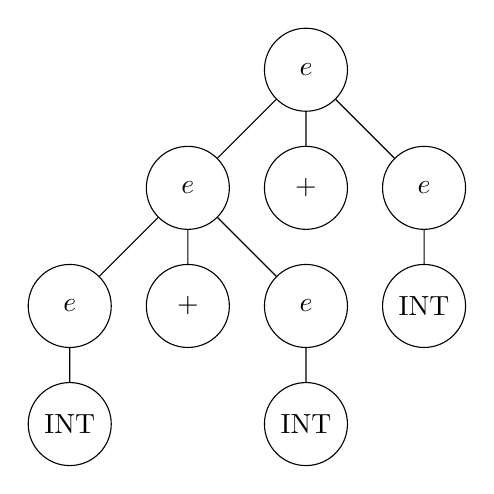
\begin{tikzpicture}
  \tikzstyle{every node}=[circle, draw, minimum size=3em]
  \node {$e$}
    child { node {$e$} 
      child { node {$e$} child { node{\lstinline{INT}} }
      }
      child { node {$+$} }
      child { node {$e$} child { node{\lstinline{INT}} }}
    }
    child { node {$+$} }
    child { node {$e$} child { node{\lstinline{INT}} }};
\end{tikzpicture}
\end{center}

Can we do a different leftmost derivation?
\end{frame}
%%%%%%%%%%%%%%%%%%%%%%%%%%%%%%%%%%%%%%%%%%%%%%%%%%%%%%%%%%%%%%%%%%%%%%%%%%%%%%%%

%%%%%%%%%%%%%%%%%%%%%%%%%%%%%%%%%%%%%%%%%%%%%%%%%%%%%%%%%%%%%%%%%%%%%%%%%%%%%%%%
\begin{frame}
\frametitle{BNF Leftmost Derivaion Answer (2)}

\begin{align*}
e &\Rightarrow e + e\\
  &\Rightarrow \text{\lstinline{INT}} + e\\
  &\Rightarrow \text{\lstinline{INT}} + e + e\\
  &\Rightarrow \text{\lstinline{INT}} + \text{\lstinline{INT}} + e\\
  &\Rightarrow \text{\lstinline{INT}} + \text{\lstinline{INT}} +
               \text{\lstinline{INT}}
\end{align*}

And the parse tree?
\end{frame}
%%%%%%%%%%%%%%%%%%%%%%%%%%%%%%%%%%%%%%%%%%%%%%%%%%%%%%%%%%%%%%%%%%%%%%%%%%%%%%%%

%%%%%%%%%%%%%%%%%%%%%%%%%%%%%%%%%%%%%%%%%%%%%%%%%%%%%%%%%%%%%%%%%%%%%%%%%%%%%%%%
\begin{frame}
\frametitle{Parse Tree Answer (2)}

\begin{center}
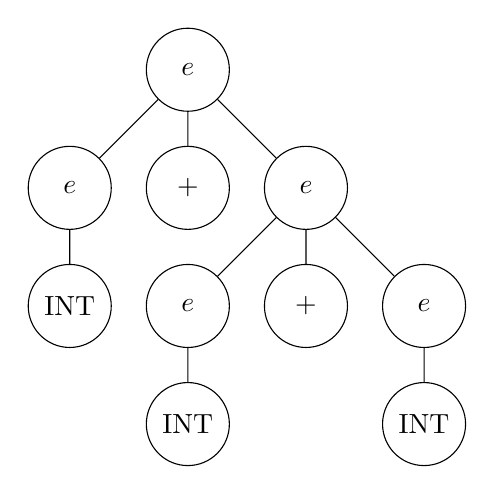
\begin{tikzpicture}
  \tikzstyle{every node}=[circle, draw, minimum size=3em]
  \node {$e$}
    child { node {$e$} child { node{\lstinline{INT}} }}
    child { node {$+$} }
    child { node {$e$} 
      child { node {$e$} child { node{\lstinline{INT}} }}
      child { node {$+$} }
      child { node {$e$} child { node{\lstinline{INT}} }}
    };
\end{tikzpicture}
\end{center}
\end{frame}
%%%%%%%%%%%%%%%%%%%%%%%%%%%%%%%%%%%%%%%%%%%%%%%%%%%%%%%%%%%%%%%%%%%%%%%%%%%%%%%%

%%%%%%%%%%%%%%%%%%%%%%%%%%%%%%%%%%%%%%%%%%%%%%%%%%%%%%%%%%%%%%%%%%%%%%%%%%%%%%%%
\begin{frame}
\frametitle{Ambiguity}

If any of the inputs has more than one leftmost derivation the \alert{grammar}
is called \alert{ambiguous}\\~\\

You do not want any ambiguity in your grammar
\end{frame}
%%%%%%%%%%%%%%%%%%%%%%%%%%%%%%%%%%%%%%%%%%%%%%%%%%%%%%%%%%%%%%%%%%%%%%%%%%%%%%%%

%%%%%%%%%%%%%%%%%%%%%%%%%%%%%%%%%%%%%%%%%%%%%%%%%%%%%%%%%%%%%%%%%%%%%%%%%%%%%%%%
\begin{frame}[plain, noframenumbering]
  \begin{beamercolorbox}[wd=\paperwidth, sep=2em]{solarizedcolorbox}
    {\usebeamerfont{title}\usebeamercolor[fg]{title}End Parsing}
  \end{beamercolorbox}
\end{frame}
%%%%%%%%%%%%%%%%%%%%%%%%%%%%%%%%%%%%%%%%%%%%%%%%%%%%%%%%%%%%%%%%%%%%%%%%%%%%%%%%
\end{document}
